\documentclass[../../../../main.tex]{subfiles}
\begin{document}

\section{User Input}
Back when designing prototype 1 I talked about the idea of a class that essentially stores data that different parts of the program can access. The reason for this is to remove the reason for global variables which are bad practice.
\subsection{Shared Layer Access}
The shared layer access will be a way for the input method to give layers to the plot pane to then add to its layers. It will contain an attribute that is the dictionary type data structure to hold all of the layers. This is so that a specific layer can be identified and removed (if the user wishes to remove a function). It will also contain public methods to add and remove layers from the list, and a getter for the dictionary values (the plotpane doesn't need the identifiers) in the form of a list so that the plotpane can access the list to use. It will also contain a property that is connected to the plotpane that will notify when the list has changed so that the plotpane can draw again. Here is the class diagram for the Shared Layer Access class:
\begin{figure}[H]
	\centering
	\includegraphics[width=0.7\textwidth]{diagrams/sharedLayer.mps}
	\caption{Shared Layer Access Class}
\end{figure}
\newpage
\subsection{Input Method}
There are two parts to this input. I will have a miniature pane to input and control individual functions, which I will call an expression box, and then a scroll pane to store all these expression boxes. The reason I am using a scroll pane for this is because if you keep adding expression boxes I want the user to be able to scroll down to see all off them.
\subsubsection{Input Pane}
The input pane will store all the expression boxes and it will have a button to add a new box. This is how it will look like:
\begin{figure}[H]
	\centering
	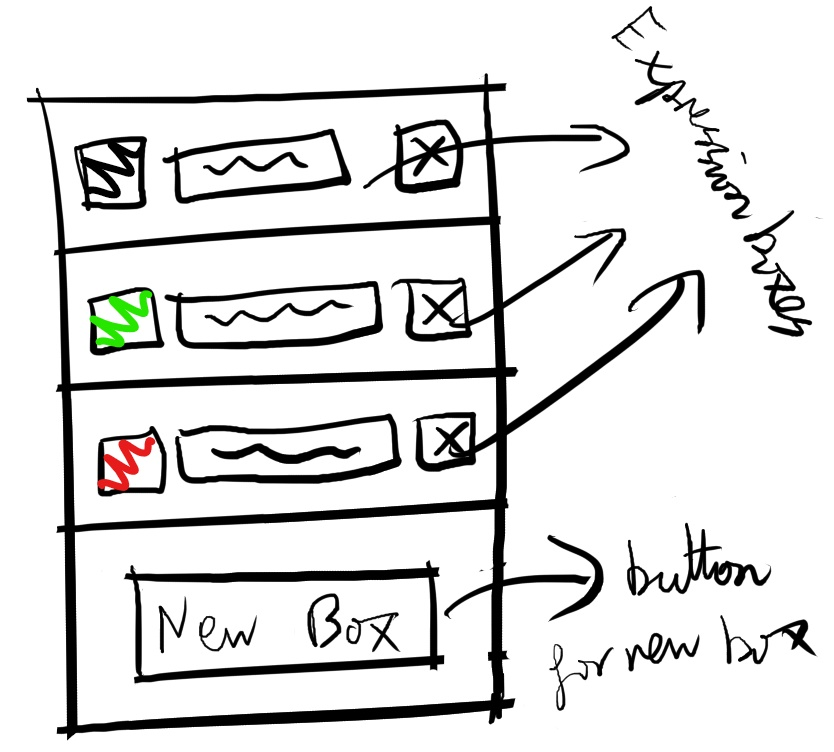
\includegraphics[width=0.5\textwidth]{images/inputPane}
	\caption{Input Pane}
\end{figure}
From an implementation point of view I will just create a class that will inherit scroll pane. This allows it to mesh with the rest of the program, and is feasible to do without a GUI builder since it is quite a simple design. I will need some way to identify each expression box to be able to remove and update the function/layer associated with it. I will do this through an attribute of type integer called \texttt{ID}. I will simply use an attribute within the input pane class to keep track of what the next ID is to assign the next expression box. I will automatically make each function a new colour and this will be done with an array that will contain the standard colours that I will use and each new expression box will cycle through each of them.\\
\newpage
\subsubsection{Expression Box}
I will make the expression box look similar to the one in Desmos shown below.
\begin{figure}[H]
	\centering
	
\includegraphics[width=0.6\textwidth]{images/desmos}
	\caption{Input in Desmos}
\end{figure}
I made my design more simplistic and fit the theme of my program. It is shown below:
\begin{figure}[H]
	\centering
	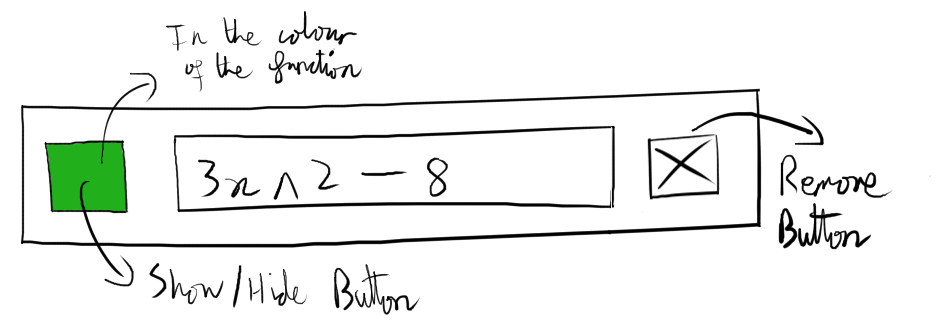
\includegraphics[width=0.8\textwidth]{images/expressionBox}
	\caption{Expression Box}
\end{figure}
I showed Lewis, a stakeholder, this design and he loved it. He said that \textit{``It looks really easy to use and I like the look.''}.\\
From an implementation point of view, I will create the expression box in FXML and then use a controller class to implement the methods to remove itself and add functions to the plot through the shared layer class. It will have an attribute called ID, to identify itself, this will be explained in the next section. It will also have an attribute for the colour of the function that it will draw.
\newpage

\end{document}